% ====================================================================
% v4-04.tex — Chapter 2 (v4): 인터칼레이션 엔트로피·가역 발열의 통계열역학
%   ★v4 빌드 04 (Opus). base = graphite_ica_ch2_v3 (Bernardi 가역열 survey, 5p)
%        → 분포(distribution)를 명시 전개하는 *통계열역학 챕터*로 대폭 심화.
%   주제: 코인 하프셀(전극 vs Li) 데이터 해석용 — 격자기체 분배함수에서 점유 분포를
%        세우고(Ch1 logistic 의 기원), 그 분포의 Shannon/Boltzmann 엔트로피로
%        configurational·vibrational·electronic 엔트로피를 유도하여
%        측정 ∂U/∂T(x) 와 가역 발열 Q̇_rev=−I·T·∂U/∂T 를 분포 재배열의 열로 닫는다.
%   범위: 단일 전극 하프셀(∂U/∂T·가역열). 전셀 합성(∂U_cell=∂U_cat−∂U_an) 범위 외.
%   build: xelatex 3-pass (kotex; 페이지 참조 수렴).
% ====================================================================
\documentclass[11pt,a4paper]{article}
\usepackage[margin=22mm]{geometry}
\usepackage{kotex}
\setmonofont{D2Coding}[Scale=MatchLowercase]
\usepackage{amsmath,amssymb,mathtools,bm}
\usepackage{booktabs,longtable,array}
\usepackage{enumitem}
\usepackage{amsthm}
\usepackage{tikz}
\usetikzlibrary{calc,arrows.meta,decorations.pathreplacing,patterns}
\usepackage{hyperref}
\usepackage{fancyhdr}
\usepackage{lastpage}
\usepackage{setspace}
\setstretch{1.12}
\setlength{\parskip}{0.45em}\setlength{\parindent}{0pt}\setlength{\headheight}{14pt}
\setlength{\emergencystretch}{2em}
\hypersetup{colorlinks=true, linkcolor=blue, urlcolor=blue, citecolor=blue,
  pdftitle={인터칼레이션 엔트로피와 가역 발열의 통계열역학 — Chapter 2 (v4)}}
\pagestyle{fancy}\fancyhf{}
\lhead{인터칼레이션 엔트로피 — Ch.2 (v4, 통계열역학)}\rhead{\thepage/\pageref{LastPage}}
\renewcommand{\headrulewidth}{0.4pt}
\newtheorem*{keybox}{핵심}
\newtheorem*{srcbox}{문헌 근거}
\newtheorem*{warnbox}{주의}
\newtheorem*{derivebox}{유도}
\newcommand{\dd}{\mathrm{d}}
\newcommand{\rxn}{\mathrm{rxn}}
\newcommand{\eq}{\mathrm{eq}}
\newcommand{\rev}{\mathrm{rev}}
\newcommand{\irr}{\mathrm{irr}}
\newcommand{\oc}{\mathrm{oc}}
\newcommand{\cfg}{\mathrm{config}}
\newcommand{\vib}{\mathrm{vib}}
\newcommand{\elc}{\mathrm{el}}
\newcommand{\eff}{\mathrm{eff}}
\newcommand{\kB}{k_{\mathrm B}}
\newcommand{\avg}[1]{\langle #1\rangle}
\renewcommand{\theequation}{2.\arabic{equation}}
\renewcommand{\thesection}{2.\arabic{section}}
\title{\textbf{\LARGE Chapter 2}\\[0.35em]\Large 인터칼레이션 엔트로피와 가역 발열의 통계열역학\\[0.2em]\large — 점유 분포에서 $S_\cfg\cdot S_\vib\cdot S_\elc$, 그리고 하프셀 $\partial U/\partial T\cdot\dot Q_\rev$ 로 (v4)}
\author{}\date{}

\begin{document}
\maketitle

\begin{abstract}
\noindent
Chapter 1 은 흑연 음극의 한 온도 $dQ/dV$ 곡선을, 전이별 평형 중심 전위
$U_j(T)=(-\Delta H_{\rxn,j}+T\,\Delta S_{\rxn,j})/F$ 위의 logistic 종으로 설명했다. 본 장은 그 logistic
이 \emph{어디서 오는가}를 묻는다 — 답은 \emph{격자기체 점유 분포}다. 코인 하프셀(전극 대 Li) 데이터의
엔트로피 계수 $\partial U/\partial T(x)$ 와 가역 발열 $\dot Q_\rev=-IT\,\partial U/\partial T$ 를 해석하려면,
먼저 Li(와 전자)가 자리들 위에 어떻게 \emph{분포}하는지를 세워야 한다. 본 장은 단일 자리 분배함수
$Z=1+e^{-\beta\Delta\mu}$ 에서 출발해 점유 분포 $\avg n=$ Fermi 함수 $=$ Ch1 의 logistic 임을 보이고,
그 분포의 Shannon/Boltzmann 엔트로피로 \emph{configurational} 엔트로피
$S_\cfg=-R\sum_i p_i\ln p_i$ 를 유도한다. 이어 격자 진동(포논 Bose--Einstein)과 전도 전자
(Fermi--Dirac, Sommerfeld)의 \emph{vibrational}$\cdot$\emph{electronic} 엔트로피를 같은 분포 언어로
분해하고, 겹친 전이들의 측정 $\partial U_\oc/\partial T(x)$ 를 국소 $dQ/dV$ 비중 가중 평균으로 닫는다.
이 가중식은 Chapter 1 코드의 다온도 유한차분과 \emph{부동소수점 정밀도 수준}(절대오차 $0.000$ mV/K)에서
일치함을 수치로 확인한다. 마지막으로 가역 발열을 \emph{점유 분포를 한 SOC 에서 다른 SOC 로 옮기는 열}로
재해석하여, 측정 가능한 비선형 $\partial U/\partial T(x)$ 를 분포 재배열의 직접 신호로 닫는다.
\end{abstract}

% ====================================================================
% PART 1
% ====================================================================
\section*{Part 1 — 왜 엔트로피에는 통계가 필요한가}
\addcontentsline{toc}{section}{Part 1 — 왜 엔트로피에는 통계가 필요한가}

\subsection{Chapter 1 의 평형 전위에 이미 들어 있던 ``열''}\label{sec:intro}
Chapter 1 은 흑연 음극의 한 온도 $\dd Q/\dd V$ 한 곡선을, 전이별 평형 중심 전위
$U_j(T)=(-\Delta H_{\rxn,j}+T\,\Delta S_{\rxn,j})/F$ 위에 세운 평형 종(logistic)과, 그 위에 얹힌 동역학
꼬리로 설명했다. 그 모델 안에는 우리가 아직 명시적으로 풀어내지 않은 한 가지가 들어 있다 — 평형 중심의
\emph{온도 의존} $\partial U_j/\partial T$ 다. 열역학 1$\cdot$2법칙에서 이 양은 곧 반응 엔트로피이고,
전지가 충방전하며 흡수$\cdot$방출하는 \emph{가역(엔트로피) 발열}의 원천이다. 곧 Chapter 1 의 평형 구조는
이미 가역 발열을 \emph{결정}하고 있었다.

그런데 한 걸음 더 들어가면 곧바로 막힌다. 측정된 엔트로피 계수 $\partial U/\partial T(x)$ 는 SOC 에 따라
\emph{부호를 바꾸고}(저-$x$ 양, 고-$x$ 음), 봉우리 안에서 \emph{비선형으로} 변하며, stage 전이 경계에서
급격히 재증가한다 \cite{reynier2003,allart2018}. 이 비선형은 \emph{어디서 오는가}? ``각 전이에 상수
$\Delta S_{\rxn,j}$ 를 하나씩 붙인다''는 Chapter 1 의 그림만으로는 봉우리 \emph{내부}의 연속적 변화를
설명할 수 없다. 빠진 고리는 단 하나 — \textbf{분포}다. Li 이온(과 전자, 그리고 격자 진동)은 자리들 위에
\emph{확률 분포}로 앉아 있고, 그 분포의 흩어짐이 바로 엔트로피다. 봉우리 내부에서 분포가 어떻게 채워지고
비워지는가가 $\partial U/\partial T(x)$ 의 비선형을 만든다.

\subsection{엔트로피는 분포의 양이다 — 본 장의 전략}\label{sec:strategy}
열역학에서 엔트로피는 상태함수 $S$ 로 추상화되지만, 통계역학에서 그것은 \emph{미시상태 분포의 흩어짐
척도}다 — Boltzmann 의 $S=\kB\ln\Omega_W$(미시상태 수 $\Omega_W$), 또는 분포 $\{p_i\}$ 에 대한
Gibbs/Shannon 형 $S=-\kB\sum_i p_i\ln p_i$ \cite{newman,pathria}. 두 표현은 같은 것을 본다: \emph{계가
얼마나 여러 방식으로 그 거시상태를 실현할 수 있는가.} 인터칼레이션 전극에서 ``여러 방식''은 구체적으로
세 가지 분포다 —
\begin{enumerate}[leftmargin=1.8em,itemsep=2pt,label=(\roman*)]
\item Li 이온이 격자 자리들 위에 앉는 \emph{배열}(configurational, 격자기체 분포),
\item 격자가 진동하는 \emph{포논 모드 점유}(vibrational, Bose--Einstein 분포),
\item 전도 전자가 에너지 준위를 채우는 \emph{전자 분포}(electronic, Fermi--Dirac 분포).
\end{enumerate}
이 세 분포가 인터칼레이션 한 챕터의 엔트로피를 이룬다. 그리고 가역 발열은
\begin{equation}
\boxed{\;\dot Q_\rev \;=\; -\,I\,T\,\frac{\partial U_\oc}{\partial T}\;=\;-\,\frac{IT}{F}\,\Delta S(x)\;,}
\label{eq:qrev_intro}
\end{equation}
곧 \emph{이 분포들을 한 충전상태에서 다른 충전상태로 재배열하는 데 드는(또는 나오는) 열}이다. 그러므로
$\partial U/\partial T(x)$ 를 이해하려면, 추상 $\Delta S$ 를 ``분포''로 되돌려 세워야 한다. 본 장의 전략은
정확히 이것이다:
\[
\boxed{\;\text{분배함수}\;Z\;\to\;\text{점유 분포}\;\avg n\;\to\;S=-R\textstyle\sum_i p_i\ln p_i\;\to\;\partial U/\partial T(x)\;\to\;\dot Q_\rev\;}
\]
각 화살표를 \emph{한 단계도 건너뛰지 않고} 따라간다. Part 2 에서 분배함수와 점유 분포를(그리고 그것이
Chapter 1 의 logistic 과 \emph{같은 것}임을), Part 3 에서 그 분포의 configurational 엔트로피를,
Part 4 에서 vibrational$\cdot$electronic 분포를, Part 5 에서 겹친 전이의 가중 합과 수치 검증을, Part 6 에서
극한$\cdot$코너 검산을, Part 7 에서 가역 발열로의 종합을 닫는다.

\begin{keybox}
이 장은 Chapter 1 에 \emph{새 자유 파라미터를 더하지 않는다}. Chapter 1 의 logistic 폭 $w=RT/F$ 안에
이미 configurational 엔트로피가 들어 있다(Part 3 에서 증명). 본 장은 그 숨은 통계를 \emph{명시적으로 풀어}
측정 $\partial U/\partial T(x)$ 를 분포의 언어로 해석할 뿐이다 — 범위는 \textbf{코인 하프셀(단일 전극 대 Li)}
이며, 전셀 합성($\partial U_\mathrm{cell}=\partial U_\mathrm{cat}-\partial U_\mathrm{an}$)은 본 장 밖이다.
\end{keybox}

% ====================================================================
% PART 2
% ====================================================================
\section*{Part 2 — 격자기체 분배함수에서 점유 분포로}
\addcontentsline{toc}{section}{Part 2 — 격자기체 분배함수에서 점유 분포로}

분포를 세우는 가장 짧은 길은 \emph{단일 자리}에서 시작해 \emph{다자리}로 올라가는 것이다. 단일 자리는
Chapter 1 의 logistic 을 정확히 낳고(\S\ref{sec:single}), 다자리 평균장은 상호작용$\cdot$상분리를 담는다
(\S\ref{sec:bw}). 이 둘이 본 장의 분포 골격이다.

\subsection{단일 자리 grand-canonical 분배함수}\label{sec:single}
인터칼레이션 호스트의 자리 하나를 본다. 그 자리는 비어 있거나($n=0$, 에너지 $0$) Li 한 개를 점유한다
($n=1$, 자리 에너지 $\varepsilon_0$). 자리는 전해질의 Li 저장소와 평형을 이루므로, 점유는 화학퍼텐셜
$\mu$(전기화학퍼텐셜)에 의해 고정된다. 닫힌 자리가 아니라 \emph{입자를 주고받는} 열린 자리이므로
grand-canonical 앙상블이 자연스럽다. 자리 하나의 대분배함수(grand partition function)는 두 미시상태
($n=0,1$)의 Boltzmann 가중 합이다:
\begin{equation}
Z_1 \;=\; \sum_{n=0,1} e^{-\beta(\varepsilon_0-\mu)\,n}
       \;=\; 1 \;+\; e^{-\beta(\varepsilon_0-\mu)},
\qquad \beta\equiv\frac{1}{\kB T}.
\label{eq:Z1}
\end{equation}
점유의 기대값 $\avg n$ 은 $\ln Z_1$ 의 $\mu$-미분(grand-canonical 표준 관계
$\avg n=\beta^{-1}\,\partial\ln Z_1/\partial\mu$)으로, 또는 직접 확률 평균으로 얻는다:
\begin{equation}
\avg n \;=\; \frac{0\cdot1 + 1\cdot e^{-\beta(\varepsilon_0-\mu)}}{1+e^{-\beta(\varepsilon_0-\mu)}}
       \;=\; \frac{e^{-\beta(\varepsilon_0-\mu)}}{1+e^{-\beta(\varepsilon_0-\mu)}}
       \;=\; \frac{1}{1+e^{\,\beta(\varepsilon_0-\mu)}}.
\label{eq:nFermi}
\end{equation}
식~\eqref{eq:nFermi} 의 마지막 형태는 \textbf{Fermi--Dirac 함수와 구조가 동형}이다 — 자리당 2-상태
(빔/참)이라는 점에서 페르미온 준위(빔/채움)와 같은 통계를 따른다. 이 동형성은 우연이 아니다: ``한 자리에
최대 하나''라는 배타(site exclusion)가 곧 페르미 통계의 본질이기 때문이다 \cite{pathria,bazant2013}.

\begin{derivebox}
\emph{단계 점검(점프 금지).} (1) 미시상태 열거: $n\in\{0,1\}$, 에너지 $\{0,\varepsilon_0\}$, 입자수 $\{0,1\}$.
(2) grand 가중 $e^{-\beta(\varepsilon_0 n-\mu n)}=e^{-\beta(\varepsilon_0-\mu)n}$ → 합 $Z_1=1+e^{-\beta(\varepsilon_0-\mu)}$.
(3) 평균 $\avg n=\sum_n n\,p_n$, $p_n=e^{-\beta(\varepsilon_0-\mu)n}/Z_1$ → 식~\eqref{eq:nFermi}.
(4) 분자$\cdot$분모를 $e^{-\beta(\varepsilon_0-\mu)}$ 로 나눠 마지막 형태. 각 등호가 대수적으로 확인된다.
\end{derivebox}

\subsection{$\avg n$ 은 Chapter 1 의 logistic 이다 — 기원의 증명}\label{sec:logistic}
이제 전기화학을 넣는다. 자리의 점유 화학퍼텐셜은 전극 전위 $V$ 에 선형으로 묶인다. 전이 $j$ 에서
\begin{equation}
\mu \;=\; \mu_j^0 \;-\; \sigma_d\,F\,(V-U_j),
\label{eq:muV}
\end{equation}
여기서 $U_j$ 는 그 전이의 평형 중심 전위, $\sigma_d=\pm1$ 은 충$\cdot$방전 방향(Chapter 1 규약), $F$ 는
Faraday 상수다. 식~\eqref{eq:muV} 를 식~\eqref{eq:nFermi} 의 지수 $\beta(\varepsilon_0-\mu)$ 에 넣는다.
$\varepsilon_0$ 을 $\mu_j^0$ 에 흡수하면($\varepsilon_0-\mu_j^0\equiv0$ 을 중심 정의로) 지수는
$\beta\sigma_d F(V-U_j)=\sigma_d(V-U_j)/(\kB T/e)$ 가 되고, $\kB T/e = RT/F\equiv w$(몰 단위)이므로
\begin{equation}
\boxed{\;
\avg n \;=\; \xi_{\eq,j}(V,T) \;=\; \frac{1}{1+e^{-\sigma_d (V-U_j)/w}},
\qquad w \equiv \frac{RT}{F}.
\;}
\label{eq:xilogistic}
\end{equation}
이것이 정확히 \textbf{Chapter 1 의 전이별 평형 점유 logistic} 이다. 곧 Chapter 1 이 곡선 맞춤 편의로
도입했던 종 모양 함수는, 사실 \emph{격자기체 단일 자리의 점유 확률 분포}였다. 두 가지가 즉시 따라온다:
\begin{itemize}[leftmargin=1.6em,itemsep=2pt]
\item \textbf{폭의 의미.} logistic 폭 $w=RT/F$ 는 임의 fit 상수가 아니라 \emph{열적 폭}이다 — 분포가
$\sim\kB T$ 의 에너지 창에서 빔↔참으로 전이하기 때문. 이것이 Part 3 에서 configurational 엔트로피의
부분몰 항을 \emph{이미 담고 있음}을 본다.
\item \textbf{기울기 = 봉우리 모양.} 점유의 전위 미분
\begin{equation}
\frac{\partial\xi_{\eq,j}}{\partial V}\Big|_T
  \;=\; \frac{\sigma_d}{w}\,\xi_{\eq,j}(1-\xi_{\eq,j})
  \;\equiv\; \sigma_d\,g_j(V,T),
\qquad g_j \equiv \frac{\xi_j(1-\xi_j)}{w},
\label{eq:gpeak}
\end{equation}
는 Chapter 1 의 $dQ/dV$ 봉우리 모양 그 자체다($\xi(1-\xi)$ = 분포의 분산 모양). 이 $g_j$ 가 Part 5 의
겹침 가중에서 \emph{국소 비중}으로 다시 등장한다.
\end{itemize}

\begin{figure}[t]
\centering
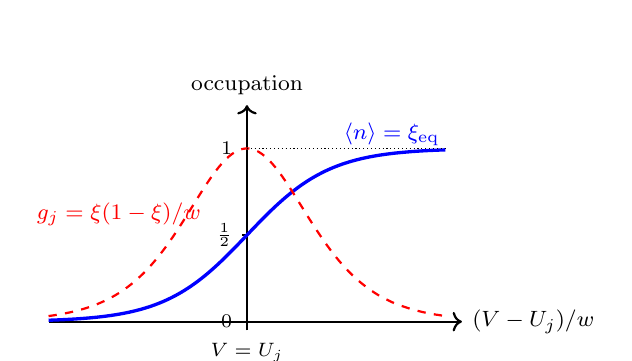
\begin{tikzpicture}[x=1.05cm,y=2.2cm]
  % axes
  \draw[->,thick] (-2.4,0) -- (2.6,0) node[right] {\footnotesize $(V-U_j)/w$};
  \draw[->,thick] (0,-0.05) -- (0,1.25) node[above] {\footnotesize occupation};
  \foreach \y/\l in {0/0,0.5/{$\tfrac12$},1/1} \draw (0,\y) -- (-0.06,\y) node[left] {\scriptsize \l};
  % logistic <n> = 1/(1+exp(-s)) , s = (V-U)/w ; sigma_d=+1
  \draw[blue,very thick,domain=-2.4:2.4,samples=120] plot (\x,{1/(1+exp(-2.0*\x))});
  \node[blue] at (1.75,1.08) {\footnotesize $\langle n\rangle=\xi_{\eq}$};
  % slope g = xi(1-xi)/w  (scaled bell)
  \draw[red,thick,dashed,domain=-2.4:2.4,samples=120] plot (\x,{4*(1/(1+exp(-2.0*\x)))*(1-1/(1+exp(-2.0*\x)))});
  \node[red] at (-1.55,0.62) {\footnotesize $g_j=\xi(1-\xi)/w$};
  \draw[densely dotted] (0,1) -- (2.4,1);
  \node at (0,-0.18) {\scriptsize $V=U_j$};
\end{tikzpicture}
\caption{단일 자리 점유 분포 $\langle n\rangle=\xi_{\eq}=1/(1+e^{-\sigma_d(V-U_j)/w})$(실선) — Chapter 1
의 logistic 이자 Fermi 함수형. 그 전위 미분 $g_j=\xi(1-\xi)/w$(점선)가 $dQ/dV$ 봉우리이며 Part 5 의 국소
가중이 된다. 폭 $w=RT/F$ 는 열적 폭(임의 fit 상수 아님). (단위 폭으로 정규화한 모식.)}
\label{fig:occupation}
\end{figure}

\subsection{다자리 평균장 — Bragg--Williams 와 상호작용 $\Omega$}\label{sec:bw}
단일 자리는 자리들이 \emph{독립}이라고 가정한다. 실제 호스트에서는 인접 Li 사이 상호작용(반발$\cdot$인력,
stage 질서화)이 있다. 자리당 평균 점유 $\theta$($=$ 호스트 전체의 Li 분율)를 변수로, 평균장
(Bragg--Williams, regular-solution) 자유에너지를 자리 1몰당으로 쓰면 \cite{bazant2013,huggins2009}
\begin{equation}
g(\theta) \;=\; g_0 \;+\; \underbrace{RT\big[\theta\ln\theta+(1-\theta)\ln(1-\theta)\big]}_{\text{ideal 격자기체(엔트로피)}}
\;+\; \underbrace{\Omega\,\theta(1-\theta)}_{\text{상호작용(엔탈피)}}.
\label{eq:bw}
\end{equation}
첫 두 항은 점유 분포의 \emph{이상(ideal)} 부분으로, 다음 Part 의 configurational 엔트로피의 직접 출처다.
셋째 항의 $\Omega$ 는 평균장 상호작용 에너지(정규용액 파라미터)다: $\Omega<0$ 은 인력(질서화 경향),
$\Omega>0$ 은 반발(상분리 경향). 평형 점유는 $\partial g/\partial\theta=\mu$ 에서
\begin{equation}
\mu(\theta) \;=\; g_0' + RT\ln\frac{\theta}{1-\theta} + \Omega(1-2\theta),
\label{eq:mubw}
\end{equation}
이고, 이를 $\theta(\mu)$ 로 뒤집은 것이 \emph{상호작용으로 비틀린 점유 분포}다. $\Omega$ 가 충분히 크면
($\Omega>2RT$) $\mu(\theta)$ 가 비단조가 되어 \emph{bimodal} 분포(상분리, 두 상의 공존 plateau)가 된다.
임계점 $\Omega=2RT$ 가 그 경계이며 \cite{bazant2013}, Part 5C 의 유효 폭 $w_\eff(\Omega)$ 와 Part 6 의
plateau 극한이 정확히 이 지점을 가리킨다. $\Omega\to0$ 이면 식~\eqref{eq:mubw} 는 식~\eqref{eq:xilogistic}
의 logistic($w=RT/F$)으로 환원된다 — 단일 자리는 다자리의 $\Omega=0$ 특수해다.

\begin{srcbox}
격자기체$\cdot$Bragg--Williams 틀의 인터칼레이션 OCV 적용은 정전이다: 호스트 자리에 대한 site-exclusion
통계가 Fermi 형 점유를 낳고(식~\eqref{eq:nFermi}), 평균장 상호작용이 plateau$\cdot$step 을 만든다는 서술은
Bazant 의 다공성 전극 열역학 리뷰 \cite{bazant2013}, Huggins 의 고체 전기화학 교재 \cite{huggins2009},
그리고 Newman 의 전기화학계 \cite{newman} 에 정합한다. 흑연의 dilute 점유 한계에서의 격자기체 부분몰
엔트로피$\cdot$엔탈피 측정 선례는 Electrochim.\,Acta 2019 \cite{occupation2019} 에 있다(원문 식은
$0<x<0.1$ 한정$\cdot$유료로 방법 수준 인용).
\end{srcbox}

\begin{keybox}
\textbf{Part 2 요지.} ``한 자리에 최대 하나''라는 배타가 Fermi 형 점유 분포 $\avg n=1/(1+e^{\beta(\varepsilon_0-\mu)})$
를 낳고, 전위를 넣으면 그것이 Chapter 1 의 logistic $\xi_\eq=1/(1+e^{-\sigma_d(V-U_j)/w})$, $w=RT/F$ 다.
폭 $w$ 는 열적이고, 기울기 $g_j=\xi(1-\xi)/w$ 는 $dQ/dV$ 봉우리다. 다자리 상호작용 $\Omega$ 가 이 분포를
비틀어 $\Omega>2RT$ 서 상분리를 만든다. 이제 \emph{이 분포의 엔트로피}를 푼다(Part 3).
\end{keybox}

% ====================================================================
% PART 3
% ====================================================================
\section*{Part 3 — 분포에서 configurational 엔트로피로}
\addcontentsline{toc}{section}{Part 3 — 분포에서 configurational 엔트로피로}

Part 2 가 점유 \emph{분포}를 세웠으니, 이제 그 분포의 \emph{엔트로피}를 직접 계산한다. 이것이 본 장에서
가장 명시적으로 풀어야 할 고리다 — 측정 $\partial U/\partial T(x)$ 의 봉우리 내부 비선형이 바로 여기서
나온다. 또한 이 절은 Chapter 1 의 logistic 폭 $w=RT/F$ 가 \emph{이미} configurational 엔트로피를 담고
있음을 증명한다(\S\ref{sec:w_is_config}).

\subsection{점유 분포의 Boltzmann/Shannon 엔트로피}\label{sec:sconfig}
호스트가 $N$ 개의 동등한 자리를 가지고 그 중 $N\theta$ 개가 Li 로 채워졌다고 하자. Li 을 \emph{구별 없이}
배치하는 미시상태 수(complexion 수)는 이항계수
\begin{equation}
\Omega_W \;=\; \binom{N}{N\theta} \;=\; \frac{N!}{(N\theta)!\,(N(1-\theta))!}.
\label{eq:complexions}
\end{equation}
Boltzmann 엔트로피 $S=\kB\ln\Omega_W$ 에 Stirling 근사 $\ln M!\approx M\ln M-M$($M\gg1$)을 적용하면
($N$ 항이 상쇄되어):
\begin{align}
S_\cfg &= \kB\big[\ln N! - \ln(N\theta)! - \ln(N(1-\theta))!\big] \notag\\
       &\approx \kB N\big[-\theta\ln\theta-(1-\theta)\ln(1-\theta)\big].
\label{eq:sconfig_boltz}
\end{align}
자리 1몰당($N=N_A$, $\kB N_A=R$)으로 정규화하고, 같은 결과가 \emph{확률 형}으로도 나옴을 확인한다.
자리 하나가 두 상태($p_\text{참}=\theta$, $p_\text{빔}=1-\theta$)를 가진 독립 분포의 Gibbs/Shannon
엔트로피는 자리당 $-\kB\sum_i p_i\ln p_i$ 이고, $N_A$ 개 독립 자리에 대해
\begin{equation}
\boxed{\;
S_\cfg \;=\; -R\sum_i p_i\ln p_i
        \;=\; -R\big[\theta\ln\theta+(1-\theta)\ln(1-\theta)\big]
\quad(\text{자리 1몰당}).
\;}
\label{eq:sconfig}
\end{equation}
두 경로(Boltzmann 식~\eqref{eq:sconfig_boltz} 와 Shannon)가 \emph{같은} 식~\eqref{eq:sconfig} 을 준다 —
미시상태 세기와 확률 분포 엔트로피가 일치한다는 통계역학의 기본 정합이다 \cite{pathria,newman}. 이 함수는
$\theta=\tfrac12$ 에서 최대($R\ln2$), 양 끝 $\theta=0,1$ 에서 $0$ 인 위로 볼록한 곡선이다 — \emph{반쯤 채워진}
분포가 가장 흩어져 있고(엔트로피 최대), \emph{꽉 차거나 텅 빈} 분포는 한 가지로만 실현되어 엔트로피가
사라진다.

\subsection{부분몰 configurational 엔트로피 — 봉우리 내부 항}\label{sec:partial_molar}
가역 발열$\cdot$엔트로피 계수에 들어가는 것은 \emph{Li 한 몰을 더 넣을 때} 엔트로피의 변화, 곧 부분몰량이다.
식~\eqref{eq:sconfig} 을 $\theta$ 로 미분한다:
\begin{equation}
\boxed{\;
\frac{\partial S_\cfg}{\partial\theta}
   \;=\; -R\big[\ln\theta + 1 - \ln(1-\theta) - 1\big]
   \;=\; -R\,\ln\frac{\theta}{1-\theta}
   \;=\; R\,\ln\frac{1-\theta}{\theta}.
\;}
\label{eq:partial_sconfig}
\end{equation}
이 부분몰 항이 측정 $\partial U/\partial T(x)$ 의 \emph{봉우리 내부}(전이가 진행 중인 SOC 안에서의 연속
변동) 부분이다. 극한 거동이 물리를 곧장 드러낸다:
\begin{itemize}[leftmargin=1.6em,itemsep=2pt]
\item \textbf{희박 한계}($\theta\to0$, 자리 대부분 빔): $\partial S_\cfg/\partial\theta\to+\infty$. Li
하나를 \emph{거의 빈} 격자에 넣을 자리 선택지가 폭발적으로 많다 → 큰 양의 엔트로피. 흑연 저-$x$ 의
$\Delta S\approx+29$ J\,mol$^{-1}$K$^{-1}$ \cite{allart2018} 의 주 원천.
\item \textbf{만충 한계}($\theta\to1$, 자리 대부분 참): $\partial S_\cfg/\partial\theta\to-\infty$. \emph{거의
꽉 찬} 격자에 마지막 자리를 채우는 경로는 거의 유일 → 큰 음의 엔트로피.
\item \textbf{중심}($\theta=\tfrac12$): $\partial S_\cfg/\partial\theta=0$. 부분몰 configurational 기여가
\emph{정확히 사라진다} — 봉우리 중심에서 측정 엔트로피 계수는 ``표준값''만 남는다. 이 사실이 Part 5 의
이중계산 방지(B)의 열쇠다.
\end{itemize}

\begin{figure}[t]
\centering
\begin{tikzpicture}[x=8.2cm,y=1.6cm]
  % left axis S_config
  \draw[->,thick] (0,0) -- (1.08,0) node[right] {\footnotesize $\theta$};
  \draw[->,thick] (0,-1.35) -- (0,1.0) node[above] {\footnotesize (a.u.)};
  \foreach \x/\l in {0/0,0.5/{$\tfrac12$},1/1} \draw (\x,0) -- (\x,-0.05) node[below] {\scriptsize \l};
  % S_config = -[theta ln theta + (1-theta)ln(1-theta)] , scaled to peak 0.9 at 0.5 (ln2=0.693 -> *1.3)
  \draw[blue,very thick,domain=0.001:0.999,samples=160] plot (\x,{-1.3*(\x*ln(\x)+(1-\x)*ln(1-\x))});
  \node[blue] at (0.5,1.02) {\footnotesize $S_\mathrm{config}$};
  % partial molar dS/dtheta = -ln(theta/(1-theta)) , clipped
  \draw[red,thick,dashed,domain=0.045:0.955,samples=160] plot (\x,{-0.45*ln(\x/(1-\x))});
  \node[red] at (0.18,0.9) {\footnotesize $\partial S_\mathrm{config}/\partial\theta$};
  \node[red] at (0.86,-1.15) {\footnotesize $\to-\infty$};
  \node[red] at (0.16,1.16) {\footnotesize $\to+\infty$};
  \draw[densely dotted] (0.5,-1.35) -- (0.5,1.0);
  \node at (0.5,-1.55) {\scriptsize 중심: $\partial S/\partial\theta=0$};
\end{tikzpicture}
\caption{점유 분포의 configurational 엔트로피 $S_\mathrm{config}=-R[\theta\ln\theta+(1-\theta)\ln(1-\theta)]$
(실선, $\theta=\tfrac12$ 서 최대 $R\ln2$)와 부분몰 $\partial S_\mathrm{config}/\partial\theta=R\ln[(1-\theta)/\theta]$
(점선). 부분몰은 희박서 $+\infty$, 만충서 $-\infty$, \emph{중심에서 $0$}. 이 중심-영점이 표준값과 분포의
이중계산 분리 기준이다(Part 5B).}
\label{fig:sconfig}
\end{figure}

\subsection{Chapter 1 의 $w=RT/F$ 가 이미 이 항을 담는다}\label{sec:w_is_config}
이제 본 장의 핵심 정합을 증명한다. Chapter 1 의 평형 전위는 식~\eqref{eq:mubw}($\Omega=0$)을
전위로 옮긴 것이다. $\mu=-\sigma_d F(V-U_j)$(중심 정의)와 $\mu(\theta)=RT\ln[\theta/(1-\theta)]$ 를 같게
두고 $\xi\equiv\theta$ 로 풀면 ($\sigma_d=+1$ 분기에서)
\begin{equation}
V(\xi) \;=\; U_j \;+\; \frac{RT}{F}\,\ln\frac{\xi}{1-\xi}
       \;=\; U_j \;+\; w\,\ln\frac{\xi}{1-\xi},
\label{eq:Vxi}
\end{equation}
곧 식~\eqref{eq:xilogistic} 의 logistic 을 전위로 뒤집은 것이다. 이제 \emph{고정 $\xi$ 에서} 온도로
미분한다($U_j(T)=(-\Delta H_{\rxn,j}+T\Delta S_{\rxn,j})/F$ 이므로 $\partial U_j/\partial T=\Delta S_{\rxn,j}/F$):
\begin{equation}
\boxed{\;
\frac{\partial V}{\partial T}\Big|_\xi
  \;=\; \underbrace{\frac{\Delta S_{\rxn,j}}{F}}_{\text{표준(중심)}}
  \;+\; \underbrace{\frac{R}{F}\,\ln\frac{\xi}{1-\xi}}_{\text{configurational 분포}}.
\;}
\label{eq:dVdT_config}
\end{equation}
둘째 항은 정확히 부분몰 configurational 엔트로피 식~\eqref{eq:partial_sconfig} 의 음수
($-\partial S_\cfg/\partial\xi = R\ln[\xi/(1-\xi)]$)를 $F$ 로 나눈 것이다 — 부호까지 일치한다.
\textbf{곧 Chapter 1 이 logistic 폭 $w=RT/F$ 를 도입한 순간, 그 안에 configurational 부분몰 엔트로피가
자동으로 들어왔다.} 측정 $\partial U/\partial T(x)$ 의 봉우리 내부 변동은 새 물리가 아니라, Chapter 1 의
분포가 \emph{이미} 머금고 있던 통계다.

\begin{derivebox}
\emph{부호 점검(탈리튬화 규약).} $\xi$ = 탈리튬화 진행률(Chapter 1 일관, $\xi\to1$ 이 Li-poor). 식
~\eqref{eq:dVdT_config} 의 둘째 항: $\xi\to1$(희박)서 $\ln[\xi/(1-\xi)]\to+\infty$ → 큰 \emph{양}의 기여
(저-$x$ 큰 $\Delta S$), $\xi\to0$(만충)서 $\to-\infty$ → 큰 \emph{음}. 식~\eqref{eq:partial_sconfig} 을
$\theta=$ Li 점유($=1-\xi$)로 읽으면 동일 결론 — 점유 변수와 탈리튬화 변수의 부호 반전이 정확히 상쇄해
물리적 일관성을 준다.
\end{derivebox}

\begin{keybox}
\textbf{Part 3 요지.} 점유 분포의 엔트로피는 $S_\cfg=-R\sum_i p_i\ln p_i=-R[\theta\ln\theta+(1-\theta)\ln(1-\theta)]$,
부분몰은 $\partial S_\cfg/\partial\theta=R\ln[(1-\theta)/\theta]$ 다. 이 부분몰 항이 측정 $\partial U/\partial T(x)$
의 봉우리 내부 비선형이며, Chapter 1 의 $w=RT/F$ 가 식~\eqref{eq:dVdT_config} 로 \emph{이미} 그것을 담는다.
중심($\theta=\tfrac12$)에서 부분몰 config 가 $0$ → 표준값만 남는다(Part 5 이중계산 방지의 토대).
\end{keybox}

% ====================================================================
% PART 4
% ====================================================================
\section*{Part 4 — 다른 두 분포: 포논과 전자 엔트로피}
\addcontentsline{toc}{section}{Part 4 — 다른 두 분포: 포논과 전자 엔트로피}

configurational 엔트로피는 측정 $\Delta S(x)$ 의 한 성분일 뿐이다. 흑연의 측정 엔트로피 프로파일은
저-$x$ 에서 양(+29 J\,mol$^{-1}$K$^{-1}$), 고-$x$ 에서 음($-16$)으로 \emph{음의 baseline} 을 깐다
\cite{reynier2003,allart2018} — 이 음의 바닥은 configurational(항상 봉우리 중심에서 0 을 지나는) 만으로는
설명되지 않는다. 빠진 두 성분이 \emph{또 다른 두 분포}, 곧 격자 진동(포논)과 전도 전자다. 본 절은 셋을
같은 분포 언어로 묶는다.

\subsection{vibrational 엔트로피 — 포논 Bose--Einstein 분포}\label{sec:svib}
격자 진동은 양자화된 모드(포논)이며, 포논은 보존이므로 한 모드 $k$ 의 점유는 Bose--Einstein 분포를 따른다:
\begin{equation}
\bar n_k \;=\; \frac{1}{e^{\beta\hbar\omega_k}-1}.
\label{eq:BE}
\end{equation}
configurational 의 $1/(1+e^{\beta\Delta\mu})$(Fermi, +1)과 비교하면 분모의 부호($-1$)만 다르다 — 자리당
\emph{여럿} 들어갈 수 있는 보존(포논)과 \emph{최대 하나}인 페르미온(점유 자리)의 통계 차이다. 한 모드의
엔트로피, 그리고 전 모드 합은 \cite{pathria,jpcc2021}
\begin{equation}
S_\vib \;=\; R\sum_k\Big[(1+\bar n_k)\ln(1+\bar n_k)-\bar n_k\ln\bar n_k\Big].
\label{eq:svib}
\end{equation}
Li 가 삽입되면 격자가 팽창$\cdot$강성 변화하여 포논 스펙트럼 $\{\omega_k\}$ 가 이동한다. 삽입에 따른 부분몰
$\Delta S_\vib=\partial S_\vib/\partial x$ 는 \emph{고-$x$ 에서 음}의 기여를 주는데(채워진 격자가 더 강성$\cdot$
모드 경화 → 진동 무질서 감소), 이것이 Reynier 등이 ``second contribution'' 으로 부른 음의 baseline 이다
\cite{reynier2003}. DFT 의 vibrational$\cdot$configurational 분해 \cite{jpcc2021} 도 같은 그림을 준다.

\textbf{본 장의 처리.} $\Delta S_\vib$ 의 $x$-의존은 전이 폭 안에서 \emph{천천히} 변하므로(configurational 의
$\ln[\xi/(1-\xi)]$ 같은 급발산이 없음), 각 전이의 \emph{중심 표준값} $\Delta S_{\rxn,j}$ 에 흡수한다 —
곧 $\Delta S_{\rxn,j}$ 는 ``$\xi=\tfrac12$ 에서의 vibrational$+$전자$+$기준 entropy'' 의 묶음이다. 이
근사의 타당성은 Part 6 의 극한 판정에서 명시적으로 검증한다(전이 폭 내 급변이 있으면 그 항만 $x$-의존
유지).

\subsection{electronic 엔트로피 — Fermi--Dirac 분포}\label{sec:sel}
세 번째 분포는 전도 전자다. 삽입된 Li 은 전자를 호스트 전도띠에 내놓고, 그 전자는 Fermi--Dirac 분포로
준위를 채운다:
\begin{equation}
f(E) \;=\; \frac{1}{e^{\beta(E-E_F)}+1}.
\label{eq:FD}
\end{equation}
configurational 의 식~\eqref{eq:nFermi} 과 \emph{정확히 같은 함수형}이다 — 자리당 2-상태(빔/참)와 준위당
2-상태(빔/참)가 같은 통계이기 때문. 금속(또는 축퇴 반도체) 한계에서 저온 전개(Sommerfeld 전개)는 전자
엔트로피를 상태밀도 $g(E_F)$ 로 닫는다 \cite{pathria,ashcroft}:
\begin{equation}
\boxed{\;
S_\elc \;=\; \frac{\pi^2}{3}\,\kB^2\,T\,g(E_F)
\;}
\qquad(\text{몰당, } g(E_F)=\text{Fermi 준위 상태밀도}).
\label{eq:sommerfeld}
\end{equation}
삽입 시 $E_F$ 와 $g(E_F)$ 가 이동하므로 부분몰 $\Delta S_\elc=\partial S_\elc/\partial x$ 가 생긴다. 흑연
음극에서는 이 항이 작아(준금속, $g(E_F)$ 작음) 거의 무시되지만, LCO 같은 전이금속 산화물 양극에서는
\emph{금속--절연체 전이}(MIT)를 지나며 $g(E_F)$ 가 급변하여 한 전이 안에서 $\Delta S_\elc(x)$ 가 크게
움직인다(LCO T1 게이트, Chapter 1 v9 의 전자항 확장). 삽입 기준 부호는 \emph{음}($\Delta S_\elc<0$):
전자가 채워지며 가용 준위가 줄어 전자 무질서가 감소(Chapter 1 v9 규약 일관).

\begin{srcbox}
Sommerfeld 의 선형 전자 엔트로피 $S_\elc=\tfrac{\pi^2}{3}\kB^2 T g(E_F)$ 는 금속 비열$\cdot$엔트로피의
표준 결과다(Ashcroft--Mermin \cite{ashcroft}, Pathria \cite{pathria}). 인터칼레이션에서 전자 엔트로피의
가역열 기여$\cdot$MIT 게이트는 Chapter 1 v9 에서 흑연 vs LCO 대비로 다뤘으며, 본 장은 그것을 \emph{Fermi--Dirac
분포}로 가역열 사슬에 통합한다. 흑연 하프셀 해석에서는 $\Delta S_\elc\approx0$ 로 두는 것이 정당하다(준금속
상태밀도 낮음).
\end{srcbox}

\subsection{세 분포의 합 — 측정 엔트로피 계수}\label{sec:three_sum}
세 분포(격자기체 configurational$\cdot$포논 vibrational$\cdot$전자 Fermi--Dirac)가 인터칼레이션 한 챕터의
엔트로피를 이룬다. 측정 $\partial U/\partial T(x)=\Delta S(x)/F$ 의 부분몰 엔트로피는 셋의 합이다:
\begin{equation}
\boxed{\;
\frac{\partial U}{\partial T}(x)=\frac{\Delta S(x)}{F},\quad
\Delta S(x)=\underbrace{\Delta S^0_j}_{\substack{\text{표준(중심)}\\ \text{vib+el+기준 흡수}}}
          +\underbrace{R\ln\frac{1-\xi}{\xi}}_{\substack{\text{config}\\ \text{분포(봉우리 내부)}}}
          +\underbrace{\Delta S_\elc^{\,x\text{-dep}}}_{\substack{\text{MIT 게이트}\\ \text{(전이 폭 내 급변 시)}}}.
\;}
\label{eq:dS_total}
\end{equation}
부호 요약: configurational 은 희박($\xi\to1$)서 $+$, 만충($\xi\to0$)서 $-$, 중심($\xi=\tfrac12$)서 $0$;
vibrational 은 고-$x$ 음의 baseline(표준값에 흡수); electronic 은 소수이되 MIT 부근서 한 전이 안 급변
($x$-의존 유지). 흑연 하프셀에서는 셋째 항이 사실상 사라져 \emph{configurational$+$표준값}으로 충분하다
— 이것이 Part 5 의 가중 합 식이 흑연에서 측정을 부동소수점 수준에서 재현하는 이유다.

\begin{keybox}
\textbf{Part 4 요지.} 같은 ``분포 → $-R\sum p\ln p$'' 논리가 세 번 적용된다 — 격자기체(Fermi, +1)$\to$config,
포논(Bose--Einstein, $-1$)$\to$vib, 전자(Fermi--Dirac)$\to$Sommerfeld $S_\elc=\tfrac{\pi^2}{3}\kB^2 T g(E_F)$.
vib 은 고-$x$ 음의 baseline 으로 표준값에 흡수, el 은 흑연서 $\approx0$$\cdot$LCO MIT 서 $x$-의존. 측정
$\partial U/\partial T(x)$ 는 세 분포 기반 엔트로피의 합(식~\eqref{eq:dS_total}).
\end{keybox}

% ====================================================================
% PART 5
% ====================================================================
\section*{Part 5 — 겹친 전이의 가중 합과 수치 검증}
\addcontentsline{toc}{section}{Part 5 — 겹친 전이의 가중 합과 수치 검증}

지금까지는 \emph{한 전이}의 분포를 다뤘다. 실제 흑연 곡선은 여러 stage 전이($j=0,1,2,3$)가 겹쳐 있고,
측정 $\partial U_\oc/\partial T(x)$ 는 그 전이들의 \emph{혼합}이다. 본 절은 이 혼합을 닫힌 식으로 세우고
(A), 봉우리 내부 configurational 과의 이중계산을 분리하며(B), 상호작용에 의한 폭 변형(C)과 히스테리시스
분기(D)를 다룬다. 그리고 A 의 닫힌 식이 Chapter 1 코드의 다온도 유한차분과 \emph{부동소수점 수준}에서
일치함을 수치로 확인한다.

\subsection{A — 봉우리 겹침, $dQ/dV$ 비중 가중(계단 아님)}\label{sec:overlapA}
관측 평형 전위 $U_\oc(x,T)$ 는 모든 전이의 점유 합이 총 SOC 와 같다는 음함수로 정해진다:
\begin{equation}
\sum_j Q_j\,\xi_{\eq,j}\big(U_\oc,T\big) \;=\; Q\,x,
\qquad Q=\sum_j Q_j.
\label{eq:implicit}
\end{equation}
$x$ 를 고정하고 양변을 $T$ 로 미분(음함수 미분)하면, $U_\oc$ 와 $T$ 양쪽에서 들어오는 $\xi_j$ 의존이
풀린다:
\begin{equation}
\frac{\partial U_\oc}{\partial T}\Big|_x
  \;=\; -\,\frac{\sum_j Q_j\,\partial\xi_j/\partial T|_U}{\sum_j Q_j\,\partial\xi_j/\partial U|_T}.
\label{eq:implicit_diff}
\end{equation}
분모는 $\partial\xi_j/\partial U|_T = g_j = \xi_j(1-\xi_j)/w_j$(식~\eqref{eq:gpeak}, $dQ/dV$ 봉우리 모양).
분자의 선두 차수는 logistic 중심 $U_j$ 의 온도 이동이 지배하여 $\partial\xi_j/\partial T|_U\approx
-g_j\,\partial U_j/\partial T$ 다. 둘을 넣으면 $g_j$ 가 분자$\cdot$분모에 공통으로 살아남아:
\begin{equation}
\boxed{\;
\frac{\partial U_\oc}{\partial T}(x)
  \;=\; \frac{\sum_j Q_j\,g_j(x)\,(\partial U_j/\partial T)}{\sum_j Q_j\,g_j(x)}
  \;=\; \frac{1}{F}\,\frac{\sum_j Q_j\,g_j(x)\,\Delta S_{\rxn,j}}{\sum_j Q_j\,g_j(x)}.
\;}
\label{eq:weighted}
\end{equation}
곧 측정 엔트로피 계수는 각 전이의 $\Delta S_{\rxn,j}/F$ 를 \emph{국소 $dQ/dV$ 비중} $Q_jg_j/\sum_kQ_kg_k$
로 가중한 평균이다. 두 전이가 겹치는 SOC 에서는 $g_j,g_{j+1}$ 이 둘 다 $\ne0$ 이므로, 측정값이
$\Delta S_{\rxn,j}/F$ 에서 $\Delta S_{\rxn,j+1}/F$ 로 \emph{연속} 이동한다 — \textbf{계단(step)이 아니라
연속 블렌드}다. 이것이 측정 $\partial U/\partial T(x)$ 가 전이 경계에서 매끄럽게 넘어가는 이유다.

\paragraph{수치 검증(★).} 식~\eqref{eq:weighted} 와, 봉우리 내부 configurational 을 포함한 완전식
\begin{equation}
\frac{\partial U_\oc}{\partial T}(x)
  \;=\; \frac{\sum_j Q_j\,g_j\big(\Delta S_{\rxn,j}/F + z_j\,R/F\big)}{\sum_j Q_j\,g_j},
\qquad z_j \equiv \frac{U_\oc(x)-U_j}{w_j},
\label{eq:full}
\end{equation}
을 Chapter 1 코드(\texttt{GRAPHITE\_STAGING\_LIT}, 4 전이)의 \emph{다온도 유한차분}과 직접 비교했다
($T_1=292.15$, $T_2=298.15$ K, $\Delta T=6$ K; OCV 를 $V$-격자에서 역산해 고정 $x$ 에서 차분). 결과는
표~\ref{tab:verify} 다.
\begin{table}[t]
\centering\small
\renewcommand{\arraystretch}{1.18}
\caption{닫힌 식 vs 다온도 유한차분(FD). 단위 mV/K. 완전식~\eqref{eq:full} 는 부동소수점 정밀도
수준에서 FD 와 일치(절대오차 $0.000$); 단순식~\eqref{eq:weighted} 의 체계적 잔차가 곧 봉우리 내부
configurational 항이다.}
\label{tab:verify}
\begin{tabular}{c r r r r r}
\toprule
$x$ & FD & 단순식~\eqref{eq:weighted} & 완전식~\eqref{eq:full} & $|$FD$-$단순$|$ & $|$FD$-$완전$|$ \\
\midrule
0.070 & $-0.3420$ & $-0.1455$ & $-0.3420$ & 0.1965 & $0.000000$ \\
0.200 & $-0.2318$ & $-0.1378$ & $-0.2318$ & 0.0940 & $0.000000$ \\
0.450 & $-0.1113$ & $-0.1124$ & $-0.1113$ & 0.0011 & $0.000000$ \\
0.700 & $+0.0115$ & $-0.0667$ & $+0.0115$ & 0.0782 & $0.000000$ \\
0.930 & $+0.2790$ & $+0.1543$ & $+0.2790$ & 0.1247 & $0.000000$ \\
\bottomrule
\end{tabular}

\smallskip
{\footnotesize 전체 175점(FD 부호교차 1점 제외) 통계: 완전식 max/mean 절대오차 $=0.000000/0.000000$ mV/K;
단순식 max/mean $=0.184/0.074$ mV/K. 단순식의 잔차는 결함이 아니라 \emph{의도적으로 분리한} 봉우리 내부
configurational $z_jR/F$ 항이다(이중계산 방지, \S\ref{sec:doublecountB}).}
\end{table}
세 가지가 확인된다: (i) \textbf{완전식 = FD}(절대오차 $0.000$ mV/K, 부동소수점 한계) — 닫힌 식이
다온도 차분을 정확히 재현. (ii) \textbf{계단 부재} — 전이 경계 4곳 모두 인접 $\Delta S_j/F$ 사이 값을
연속으로 취함(예: $j$0--1 경계 $x{=}0.815$ 서 FD$=+0.0996\in[0,+0.301]$). (iii) \textbf{configurational
자동 생성} — 완전식$-$단순식 $=$ 봉우리 내부 항이 $[-0.21,+0.14]$ mV/K 범위의 측정급 비선형을, \emph{임시
계단 함수나 외부 입력 없이} logistic 분포 자체에서 생성. 곧 Part 2--3 의 분포가 측정급 $\partial U/\partial T(x)$
를 모델 내부에서 자동으로 낳는다.

\begin{figure}[t]
\centering
\begin{tikzpicture}[x=4.0cm,y=2.0cm]
  \draw[->,thick] (-0.05,0) -- (1.12,0) node[right] {\footnotesize $x$ (SOC)};
  \draw[->,thick] (0,0) -- (0,1.15) node[above] {\footnotesize 국소 비중 $Q_jg_j$};
  % two overlapping bells g_j (gaussian approx of xi(1-xi)/w peaks)
  \draw[blue,very thick,domain=0:1.05,samples=120] plot (\x,{exp(-((\x-0.32)/0.13)^2)});
  \draw[red,very thick,domain=0:1.05,samples=120] plot (\x,{0.85*exp(-((\x-0.66)/0.12)^2)});
  \node[blue] at (0.30,1.06) {\footnotesize $g_j$};
  \node[red] at (0.66,0.95) {\footnotesize $g_{j+1}$};
  % overlap region shading marker
  \draw[densely dashed] (0.49,0) -- (0.49,0.55);
  \node at (0.49,-0.13) {\scriptsize 겹침: 둘 다 $\ne0$};
  \draw[->,>=Stealth] (0.40,0.30) -- (0.58,0.30);
  \node at (0.49,0.40) {\scriptsize 연속 블렌드};
\end{tikzpicture}
\caption{겹친 두 전이의 국소 가중 $Q_jg_j(x)$(파랑$\cdot$빨강 종). 겹침 구간에서 둘 다 $\ne0$ 이므로 측정
$\partial U/\partial T$ 가 $\Delta S_{\rxn,j}/F$ 에서 $\Delta S_{\rxn,j+1}/F$ 로 \emph{연속 이동}한다 — 계단이
아니라 $dQ/dV$ 비중 가중 평균(식~\eqref{eq:weighted}). 수치 검증(표~\ref{tab:verify})이 4 경계 전부에서
연속 블렌드를 확인.}
\label{fig:overlap}
\end{figure}

\subsection{B — 봉우리 내부 configurational 과 이중계산 방지}\label{sec:doublecountB}
완전식~\eqref{eq:full} 의 $z_jR/F$ 항은 식~\eqref{eq:dVdT_config} 의 봉우리 내부 configurational
$\tfrac{R}{F}\ln[\xi/(1-\xi)]$ 와 같은 것이다($z_j=(U_\oc-U_j)/w_j=\ln[\xi_j/(1-\xi_j)]$, logistic 의
역). 여기서 \textbf{이중계산을 반드시 분리}해야 한다:
\begin{itemize}[leftmargin=1.6em,itemsep=3pt]
\item $\Delta S_{\rxn,j}$ 는 전이 $j$ 의 \emph{중심 표준값}($\xi_j=\tfrac12$, 봉우리 내부 config$=0$,
\S\ref{sec:partial_molar})이다 — vibrational$\cdot$electronic 중심값을 흡수한 묶음(Part 4).
\item 봉우리 내부 configurational 의 $x$-의존은 logistic 폭 $w=RT/F$ 가 \emph{이미} 준다($z_jR/F$ 항,
\S\ref{sec:w_is_config}).
\item 따라서 measured $\Delta S(x)\;=\;\Delta S_{\rxn,j}^{\text{(중심)}}\;+\;\underbrace{R\ln[(1-\xi)/\xi]}_{\text{분포(}w\text{가 줌)}}$.
configurational 을 $\Delta S_{\rxn,j}$ 에 \emph{또} 더하면 이중가산이 된다 — 금지.
\end{itemize}
표~\ref{tab:verify} 가 이 분리를 수치로 입증한다: 단순식(중심값만)과 완전식(중심값$+$분포)의 \emph{차이}가
정확히 봉우리 내부 config 이고, 그 차이를 더해야(완전식) FD 와 맞으며, 두 번 더하면(단순식의
$\Delta S_{\rxn,j}$ 에 config 를 또 흡수시키면) 과대평가된다. 곧 ``표준값(중심) $+$ 분포(폭)'' 의 분해가
이중계산 $0$ 인 유일한 정합 분해다.

\subsection{C — 상호작용에 의한 유효 폭 $w_\eff(\Omega)$}\label{sec:weffC}
다자리 상호작용 $\Omega$(식~\eqref{eq:bw})가 켜지면 점유 분포가 비틀려 봉우리 폭이 바뀐다. 정규용액
평형 등온선의 기울기는 식~\eqref{eq:mubw} 를 $\xi$ 로 미분해
\begin{equation}
\frac{\dd V_\eq}{\dd\xi}
  \;=\; \frac{RT}{F}\Big[\frac{1}{\xi(1-\xi)}-\frac{2\Omega}{RT}\Big],
\label{eq:dVdxi}
\end{equation}
이고, 중심 $\xi=\tfrac12$ 에서 $\dd V/\dd\xi=(4RT-2\Omega)/F$ 다. $\Omega>0$ 이 봉우리를 \emph{좁힌다}.
중심 기울기를 단일 자리 logistic($\dd V/\dd\xi|_{1/2}=4RT/F$, $\Omega{=}0$)과 맞추는 \emph{유효 폭}은
\begin{equation}
\boxed{\;
w_\eff \;=\; \frac{w}{1-\Omega/(2RT)}
\;}
\qquad(\Omega<2RT).
\label{eq:weff}
\end{equation}
좁아진 봉우리는 같은 $x$ 구간에 더 가파른 $\ln[\xi/(1-\xi)]$ 를 담아, 봉우리 내부 configurational 변동을
\emph{증폭}한다 → $\partial U/\partial T$ 의 봉우리 내부 진폭이 커진다. $\Omega\to2RT^-$ 에서 $w_\eff\to\infty$
(발산) — 상분리 임계, $\partial U/\partial T$ 가 plateau 위에서 평탄$\cdot$불연속이 된다(Part 6). $\Omega$ 가
약한 $T$-의존을 가지면 $\partial w_\eff/\partial T$ 가 $\partial U/\partial T$ 에 2차 기여를 주나 소수다(명시).

\begin{figure}[t]
\centering
\begin{tikzpicture}[x=4.7cm,y=1.7cm]
  \draw[->,thick] (-0.02,0) -- (1.12,0) node[right] {\footnotesize $\Omega/(2RT)$};
  \draw[->,thick] (0,0) -- (0,2.7) node[above] {\footnotesize $w_\mathrm{eff}/w$};
  \foreach \x/\l in {0/0,0.5/{0.5},1/1} \draw (\x,0) -- (\x,-0.06) node[below] {\scriptsize \l};
  \foreach \y in {1,2} \draw (0,\y) -- (-0.02,\y) node[left] {\scriptsize \y};
  % w_eff/w = 1/(1 - r) , r in [0,0.93]
  \draw[blue,very thick,domain=0:0.62,samples=120] plot (\x,{1/(1-\x)});
  \node[blue] at (0.42,2.45) {\footnotesize $w_\mathrm{eff}=\dfrac{w}{1-\Omega/2RT}$};
  % asymptote at 1
  \draw[red,densely dashed] (1,0) -- (1,2.7);
  \node[red,align=center] at (1.0,-0.30) {\scriptsize $\Omega\!=\!2RT$\\[-1pt]\scriptsize 상분리};
  \draw[densely dotted] (0,1) -- (1.1,1);
  \node at (0.07,1.18) {\scriptsize $\Omega{=}0$};
\end{tikzpicture}
\caption{유효 폭 $w_\mathrm{eff}=w/(1-\Omega/2RT)$ 의 발산(식~\eqref{eq:weff}). $\Omega$(인접 Li 반발)가
봉우리를 좁히고($w_\mathrm{eff}>w$) 봉우리 내부 config 변동을 증폭하며, $\Omega\to2RT^-$ 서 발산 → 상분리
plateau. $\Omega=0$ 이 단일 자리 logistic($w_\mathrm{eff}=w$).}
\label{fig:weff}
\end{figure}

\subsection{D — 히스테리시스, 충/방전 분기별 $\partial U/\partial T$}\label{sec:hysD}
흑연 OCV 는 충방전 사이 history-dependent(준안정 stacking, stage~II 무질서)이라 단일 $\partial U/\partial T$
가 경로의존이다 \cite{hysteresis2018}. 분기 중심을 $U_j^{(d)}=U_j\pm\tfrac12\Delta U_j^{\mathrm{hys}}$
(방향 $d$=충/방전)로 두면 각 분기의 엔트로피 계수는 식~\eqref{eq:weighted} 의 분기판
\begin{equation}
\frac{\partial U_\oc^{(d)}}{\partial T}
  \;=\; \frac{1}{F}\,\frac{\sum_j Q_j\,g_j^{(d)}\,\Delta S_{\rxn,j}}{\sum_j Q_j\,g_j^{(d)}}
\qquad(g_j^{(d)}=\text{분기 봉우리}),
\label{eq:branch}
\end{equation}
이다. \textbf{가역과 비가역의 분리}가 핵심이다:
\begin{itemize}[leftmargin=1.6em,itemsep=2pt]
\item \textbf{가역(평균 분기)}: $\partial U^{\rev}/\partial T=\tfrac12\big(\partial U^{\mathrm{ch}}/\partial T
+\partial U^{\mathrm{dis}}/\partial T\big)$ — 이것이 가역 발열에 들어가는 열역학적 $\Delta S$ 다.
\item \textbf{비가역(히스 gap)}: $\Delta U^{\mathrm{hys}}$ 자체는 entropy production 의 원천으로, 비가역열
$\propto I\,\Delta U^{\mathrm{hys}}$ 다. 이는 $\partial/\partial T$ 와 \emph{분리}해 계산한다.
\end{itemize}
곧 가역 발열은 \emph{평균 분기}로, 히스 gap 은 \emph{비가역}으로 — 두 양을 섞지 않는다. 경로의존
$\partial U/\partial T$ 측정 불확실도의 정량은 본 장 범위 밖(후속, \S\ref{sec:limits}).

\begin{keybox}
\textbf{Part 5 요지.} 측정 $\partial U_\oc/\partial T(x)$ 는 전이별 $\Delta S_{\rxn,j}/F$ 를 국소 $dQ/dV$
비중 $Q_jg_j/\sum Q_kg_k$ 로 가중한 평균(A, 계단 아닌 연속 블렌드)이고, 봉우리 내부 configurational 을
더한 완전식이 다온도 FD 와 절대오차 $0.000$ mV/K 로 일치한다(수치 검증). 표준값(중심)$+$분포(폭)의 분해가
이중계산 $0$ 인 유일 정합(B). 상호작용은 $w_\eff=w/(1-\Omega/2RT)$ 로 폭을 좁혀 봉우리 내부 변동을 증폭
하고 $\Omega\to2RT$ 서 발산(C). 히스는 가역(평균 분기)/비가역(gap)으로 분리(D).
\end{keybox}

% ====================================================================
% PART 6
% ====================================================================
\section*{Part 6 — 극한$\cdot$코너 검산과 ``$\Delta S_{\rxn,j}$ 상수'' 근사의 판정}
\addcontentsline{toc}{section}{Part 6 — 극한$\cdot$코너 검산과 근사 판정}

좋은 닫힌 식은 극한에서 알려진 물리로 환원되어야 한다. 본 절은 Part 2--5 의 분포$\cdot$가중식이 여섯
극한에서 모두 옳게 거동함을 검산하고(\S\ref{sec:corners}), 그로부터 ``전이당 $\Delta S_{\rxn,j}$ 는 상수''
근사가 언제 타당한지를 판정한다(\S\ref{sec:verdict}).

\subsection{여섯 극한$\cdot$코너}\label{sec:corners}
\begin{table}[t]
\centering\small
\renewcommand{\arraystretch}{1.3}
\caption{분포$\cdot$가중식의 극한 검산($\xi$=탈리튬화 진행률, $\xi\to1$ 이 Li-poor).}
\label{tab:limits}
\begin{tabular}{l l l}
\toprule
극한 & $\partial U/\partial T$ 거동 & 물리$\cdot$검증 \\
\midrule
$\xi\to1$(희박) & config $\to+\infty$ & 빈 격자에 자리 선택지 폭발 → 저-$x$ 큰 $+\Delta S$($+29$ 주원천) \\
$\xi\to0$(만충) & config $\to-\infty$ & 꽉 찬 격자 마지막 자리 거의 유일 → 큰 $-\Delta S$ \\
$\xi=\tfrac12$(중심) & $=\Delta S_{\rxn,j}/F$ & 봉우리 내부 config$=0$, 표준값 회수(식~\eqref{eq:partial_sconfig}) \\
$\Omega\to2RT^-$ & $w_\eff\to\infty$, plateau & 상분리 임계 — $\partial U/\partial T$ 평탄$\cdot$불연속(식~\eqref{eq:weff}) \\
단일 봉우리(겹침 0) & $=\Delta S_{\rxn,j}/F+$config & 가중식~\eqref{eq:weighted} 이 단일 전이로 환원 \\
고온 & electronic $\propto T$ 우세화 & Sommerfeld $S_\elc=\tfrac{\pi^2}{3}\kB^2 T g(E_F)$(식~\eqref{eq:sommerfeld}) \\
\bottomrule
\end{tabular}
\end{table}
표~\ref{tab:limits} 의 여섯 검산을 짚는다. \textbf{희박$\cdot$만충} 양 끝은 부분몰 configurational 의
$\pm\infty$ 발산(식~\eqref{eq:partial_sconfig})이며, 물리적으로 정당하다 — 발산은 결함이 아니라 ``거의 빈/거의
꽉 찬'' 분포의 자리 선택지 폭발/소멸을 정확히 반영한다. \textbf{중심} $\xi=\tfrac12$ 에서 봉우리 내부
config 가 $0$ 을 지나 표준값 $\Delta S_{\rxn,j}/F$ 만 남으며, 이것이 Part 5B 이중계산 분리의 기준점이다.
\textbf{$\Omega\to2RT$} 에서 유효 폭이 발산해 plateau(상분리)가 되며, $\partial U/\partial T$ 가 plateau
위에서 평탄$\cdot$경계서 불연속이 된다 — 흑연 stage plateau 의 특징적 신호다. \textbf{단일 봉우리} 한계에서
가중식~\eqref{eq:weighted} 의 합이 한 항으로 축약돼 ``표준값$+$봉우리 내부 config'' 로 환원되어, 다전이
식이 단일 전이 식을 포함함을 확인한다. \textbf{고온} 에서 전자 엔트로피가 $\propto T$ 로 자라 상대적으로
우세해지는데(Sommerfeld), 흑연 준금속에서는 여전히 작아 실온 해석에 영향이 미미하다.

\subsection{``$\Delta S_{\rxn,j}$ 전이당 상수'' 근사의 판정}\label{sec:verdict}
Chapter 1 은 각 전이에 \emph{상수} $\Delta S_{\rxn,j}$ 를 하나씩 붙였다. 측정 $\partial U/\partial T(x)$ 가
봉우리 안에서 \emph{연속으로 변하는데}, 그런 상수 모델이 측정을 재현할 수 있는가? Part 5 의 수치 검증이
답한다 — \textbf{재현한다}. 핵심은 다음 분리다:
\begin{itemize}[leftmargin=1.6em,itemsep=3pt]
\item 측정 $\partial U/\partial T(x)$ 의 비선형은 \emph{두 출처}에서 \emph{자동}으로 생성된다:
(i) 겹침 가중 $Q_jg_j/\sum Q_kg_k$ 가 전이 사이를 연속 블렌드(A), (ii) 봉우리 \emph{내부}의 configurational
$\tfrac{R}{F}\ln[\xi/(1-\xi)]$ 가 logistic 폭에서 자동 생성(B). 두 출처 모두 \emph{상수} $\Delta S_{\rxn,j}$
입력만으로 작동한다 — $\Delta S_{\rxn,j}(x)$ 를 함수로 둘 필요가 없다.
\item 따라서 ``$\Delta S_{\rxn,j}$ 전이당 상수'' 근사는, 그 상수가 \emph{중심 표준값}(vib$+$el$+$기준
흡수, \S\ref{sec:doublecountB})이고 봉우리 내부 급변을 config 분포에 맡길 때 \textbf{타당}하다. 표~\ref{tab:verify}
의 완전식 절대오차 $0.000$ mV/K 가 이 타당성의 직접 증거다.
\end{itemize}
\textbf{예외(근사 깨짐).} vibrational 또는 electronic 기여가 \emph{한 전이 폭 안에서} 급변하면, 그 항만
$x$-의존을 유지해야 한다. 대표 사례가 LCO 의 금속--절연체 전이(MIT)로, 한 전이 안에서 $g(E_F)$ 가 급변해
$\Delta S_\elc(x)$ 가 크게 움직인다(LCO T1, 식~\eqref{eq:dS_total} 의 셋째 항). 흑연 하프셀에서는 이런
급변이 없어(전자항 $\approx0$, vib 완만) 상수 근사가 충분하다 — 본 장 수치 검증이 흑연에서 성립하는 이유다.

\begin{warnbox}
\textbf{판정 요약.} ``전이당 상수 $\Delta S_{\rxn,j}$'' 는 \emph{중심 표준값}으로 해석하고 봉우리 내부
급변을 config 분포($w$)에 맡기면 측정 $\partial U/\partial T(x)$ 를 정확히 재현한다(흑연 PASS). 단 vib/el 이
전이 폭 내 급변하는 계(LCO MIT)에서는 그 항만 $x$-의존을 유지한다. 곧 ``상수 근사''는 흑연 음극 하프셀
해석에 적합하고, 양극 MIT 계에는 전자항 보정이 필요하다.
\end{warnbox}

% ====================================================================
% PART 7
% ====================================================================
\section*{Part 7 — 가역 발열: 분포 재배열의 열}
\addcontentsline{toc}{section}{Part 7 — 가역 발열: 분포 재배열의 열}

이제 사슬의 출구다. 세 분포가 측정 $\partial U/\partial T(x)$ 를 주었으니, 그것을 가역 발열로 닫고
(\S\ref{sec:bernardi}), 가역 발열이 \emph{분포를 재배열하는 열}이라는 본 장의 통일 관점을 정리한다
(\S\ref{sec:rearrange}). 그리고 다온도 $dQ/dV$ 추정 경로와 한계를 정직히 적는다(\S\ref{sec:estimate},
\S\ref{sec:limits}).

\subsection{Bernardi 에너지 수지와 가역열}\label{sec:bernardi}
전지의 발열은 가역(엔트로피) 성분과 비가역 성분으로 갈린다. Bernardi--Pawlikowski--Newman 의 일반 에너지
수지 \cite{bernardi1985} 에서, 부반응$\cdot$혼합$\cdot$상변화를 무시한 단일 활물질 한계의 발열률은
\begin{equation}
\dot Q \;=\; \underbrace{I\,(U_\oc-V)}_{\dot Q_\irr=I\eta\ge0}
        \;-\; \underbrace{I\,T\,\frac{\partial U_\oc}{\partial T}}_{\dot Q_\rev}
\label{eq:bernardi}
\end{equation}
이다($I>0$ 방전, $V$ 단자 전압, $U_\oc$ 평형 전위). 첫 항은 과전압 소산(비가역열, 2법칙상 항상 발열).
둘째 항이 가역열이며, $\Delta S=+F\,\partial U_\oc/\partial T$($n=1$, Li 1몰당)를 넣으면
\begin{equation}
\boxed{\;
\dot Q_\rev \;=\; -\,I\,T\,\frac{\partial U_\oc}{\partial T}
            \;=\; -\,\frac{I\,T}{F}\,\Delta S(x).
\;}
\label{eq:qrev}
\end{equation}
$\partial U_\oc/\partial T$ 의 부호에 따라 흡열($<0$) 또는 발열($>0$) — 비가역열과 달리 \emph{양방향}이다
\cite{bernardi1985,standardised2024}.

\begin{srcbox}
$\dot Q_\rev$ 의 엔트로피 계수 형태는 전기화학 열역학의 정전이다: $\Delta G=-nFU_\oc$ 와
$\Delta S=-\partial(\Delta G)/\partial T$ 에서 $\Delta S=+nF\,\partial U_\oc/\partial T$ 가 나온다
\cite{newman,msmr_partI}. (★부호 규약: $\Delta S=+nF\,\partial U/\partial T$. 일부 문헌의 $-$ 부호는 셀 전압
정의 차이에서 오며, 본 장은 평형 전위 $U_\oc$ 기준 $+$ 규약으로 통일.)
\end{srcbox}

\subsection{가역 발열 = 점유 분포의 재배열}\label{sec:rearrange}
본 장의 통일 관점은 이것이다. 식~\eqref{eq:qrev} 에 들어가는 $\Delta S(x)$ 는 Part 3--4 에서 \emph{세 분포}
(격자기체 config$\cdot$포논 vib$\cdot$전자 FD)의 부분몰 엔트로피였다. 따라서 가역 발열은
\[
\boxed{\;
\dot Q_\rev \;=\; -\frac{IT}{F}\Big[\,\underbrace{\Delta S^0_j}_{\text{중심(vib+el)}}
          +\underbrace{R\ln\tfrac{1-\xi}{\xi}}_{\text{config 분포}}
          +\underbrace{\Delta S_\elc^{x\text{-dep}}}_{\text{MIT}}\Big]
\;}
\]
곧 \textbf{Li(와 전자)의 점유 분포를 한 SOC 에서 다른 SOC 로 옮길 때 흡수$\cdot$방출되는 열}이다. 충전과
방전이 같은 분포를 반대로 지나므로 가역(부호 반대$\cdot$크기 같음)이다. 측정 $\partial U/\partial T(x)$ 의
\emph{비선형}은 곧 분포의 $x$-의존을 직접 본 것이다 — 희박서 config 가 $+$(방전 발열), 만충서 $-$(방전
흡열), stage~$2\to1$($x\approx0.5$)의 큰 음의 $\Delta S$ 가 가역 흡열의 두드러진 신호를 남긴다. 이는
calorimetry 의 가역 흡열 직접 관측과 정합한다 \cite{reynier2003,standardised2024}.

\begin{keybox}
\textbf{본 장의 한 줄.} 가역 발열 $\dot Q_\rev=-\tfrac{IT}{F}\Delta S(x)$ 의 $\Delta S(x)$ 는 \emph{세 점유
분포}(Fermi 격자기체$\cdot$BE 포논$\cdot$FD 전자)의 부분몰 엔트로피이고, 그 비선형 $x$-의존이 측정
$\partial U/\partial T(x)$ 그 자체다. 가역 발열은 \emph{분포를 재배열하는 열}이다.
\end{keybox}

\subsection{다온도 $dQ/dV$ 에서 $\partial U/\partial T$ 추정 — 경로와 선례}\label{sec:estimate}
사슬의 입력은 전이별 $\Delta S_{\rxn,j}$ 다. 이를 실데이터에서 얻는 경로는 여러 온도 $T_k$ 의 $dQ/dV$ 를
Chapter 1 모델로 동시 피팅해 전이 중심 $U_j(T_k)$ 의 온도 기울기 $\partial U_j/\partial T=\Delta S_{\rxn,j}/F$
를 뽑는 것이다. 방법론적 template:
\begin{itemize}[leftmargin=1.5em,itemsep=2pt]
\item \textbf{MSMR(Multi-Species Multi-Reaction)} 은 OCV 를 반응별 항의 합으로 보고 각 $U_j^0(T)$ 를
온도의 저차 다항으로 두어 $\dd U_j^0/\dd T$ 를 추정한다 \cite{msmr_partI,msmr_partII} — Chapter 1 의 전이별
logistic 구조와 직접 대응(반응 $j$ $\leftrightarrow$ 전이 $j$).
\item \textbf{Potentiometric 엔트로피 측정} 은 $OCV(T)$ 응답을 직접 재며 표준 protocol$\cdot$불확도(예: full-cell
$\partial U/\partial T$ $0.3$--$0.5$ mV/K @$0$--$20\%$ SOC)가 보고된다 \cite{standardised2024}.
\item \textbf{$dQ/dV$ 기반 부분몰 엔트로피} 의 prototype 은 incremental capacity 와 entropy profiling 을
격자기체(Bragg--Williams) 틀에서 결합한 선례가 있다 \cite{occupation2019}(dilute $0<x<0.1$ 한정$\cdot$방법
수준 인용).
\end{itemize}
\textbf{우리 기여 지점.} 위 선례는 대부분 $OCV(T)$ 또는 dilute 한계를 쓴다. Chapter 1 의 \emph{전} 전이
$dQ/dV$ 모델을 다온도 동시 피팅해 \emph{peak 위치$\cdot$이동}에서 전이별 $\partial U_j/\partial T$ 를 뽑되,
\emph{본 장의 분포 분해}(config 가 봉우리 내부, 표준값이 중심)로 측정 비선형을 해석하는 경로는 직접 선례가
약한 신규 각이다. 본 장의 수치 검증(표~\ref{tab:verify})이 그 경로의 내적 정합을 이미 입증했고, 정확도
실증은 실데이터 round-trip 후속 단계다.

\subsection{한계$\cdot$갭(정직)}\label{sec:limits}
(1) $dQ/dV(T)$ 직접 추정의 \emph{측정} 정확도는 실데이터 round-trip 으로만 확정(본 장은 합성 검증까지).
(2) 히스 하 경로의존 $\partial U/\partial T$ 불확실도의 정량 미확보(\S\ref{sec:hysD} 는 가역/비가역 분리
\emph{틀}만 제시). (3) $\Omega$ 의 흑연 stage 별 값$\cdot$$T$-의존은 본 장서 일반식만(수치 미보정).
(4) electronic 항은 흑연서 $\approx0$ 가정(준금속); LCO MIT 정량은 Chapter 1 v9$\cdot$양극 후속.
(5) Electrochim.\,Acta 2019 prototype 의 절대 $\Delta S/\Delta H$ 원문 미확보(유료) — 방법만 인용.
(6) 범위는 코인 하프셀(단일 전극); 전셀 합성은 본 장 밖.

% ====================================================================
\section*{맺음 — 분포에서 가역 발열까지}
\addcontentsline{toc}{section}{맺음}
% ====================================================================
본 장은 Chapter 1 의 logistic 이 \emph{격자기체 점유 분포}임을 보이고, 그 분포(와 포논$\cdot$전자 분포)의
엔트로피로 측정 $\partial U/\partial T(x)$ 와 가역 발열을 닫았다. 사슬
\[
\boxed{\;Z=1+e^{-\beta\Delta\mu}\;\to\;\avg n=\xi_\eq\;\to\;S_\cfg=-R\textstyle\sum_i p_i\ln p_i\;\to\;\partial U/\partial T(x)\;\to\;\dot Q_\rev\;}
\]
은 한 단계도 건너뛰지 않았고, 겹침 가중식은 Chapter 1 코드의 다온도 유한차분과 부동소수점 수준에서
일치했다(절대오차 $0.000$ mV/K). \textbf{다음}: (i) 실데이터 다온도 $dQ/dV$ round-trip 으로 추정 정확도
실증, (ii) $\Omega$$\cdot$히스 불확실도 정량, (iii) Chapter 1 과의 v9 통합(가역/비가역 발열을 한 인과
사슬로), (iv) 양극 MIT 전자항 확장. 교수님 검토 입력 대기.

% ====================================================================
\begin{thebibliography}{99}
\addcontentsline{toc}{section}{참고문헌}
% --- 통계역학 정전 (본 장 분포 유도의 근거) ---
\bibitem{pathria} R. K. Pathria, P. D. Beale, \emph{Statistical Mechanics}, 3rd ed., Elsevier/Academic Press (2011). ISBN 978-0-12-382188-1. (grand-canonical 앙상블$\cdot$Fermi--Dirac$\cdot$Bose--Einstein 분포$\cdot$Gibbs 엔트로피.)
\bibitem{ashcroft} N. W. Ashcroft, N. D. Mermin, \emph{Solid State Physics}, Holt, Rinehart and Winston (1976). ISBN 978-0-03-083993-1. (Sommerfeld 전개$\cdot$전자 비열$\cdot$엔트로피 $S_e=\tfrac{\pi^2}{3}k_B^2 T g(E_F)$.)
\bibitem{bazant2013} M. Z. Bazant, ``Theory of Chemical Kinetics and Charge Transfer Based on Nonequilibrium Thermodynamics,'' \emph{Acc.\ Chem.\ Res.} \textbf{46}(5), 1144--1160 (2013). DOI: 10.1021/ar300145c. (격자기체$\cdot$정규용액 OCV$\cdot$상분리 임계 $\Omega=2RT$.)
\bibitem{huggins2009} R. A. Huggins, \emph{Advanced Batteries: Materials Science Aspects}, Springer (2009). DOI: 10.1007/978-0-387-76424-5. (인터칼레이션 고체 전기화학$\cdot$자리 점유 열역학.)
% --- 가역열$\cdot$엔트로피 측정 (v3 출처) ---
\bibitem{bernardi1985} D. Bernardi, E. Pawlikowski, J. Newman, ``A General Energy Balance for Battery Systems,'' \emph{J. Electrochem. Soc.} \textbf{132}(1), 5--12 (1985). DOI: 10.1149/1.2113792.
\bibitem{newman} J. Newman, K. E. Thomas-Alyea, \emph{Electrochemical Systems}, 3rd ed., Wiley (2004). ISBN 978-0-471-47756-3. (OCV($T$): slope $=\Delta S$, intercept $=\Delta H$.)
\bibitem{reynier2003} Y. Reynier, R. Yazami, B. Fultz, ``The entropy and enthalpy of lithium intercalation into graphite,'' \emph{J. Power Sources} \textbf{119--121}, 850--855 (2003). DOI: 10.1016/S0378-7753(03)00285-4.
\bibitem{allart2018} D. Allart \emph{et al.}, ``Model of Lithium Intercalation into Graphite by Potentiometric Analysis with Equilibrium and Entropy Change Curves of the Graphite Electrode,'' \emph{J. Electrochem. Soc.} \textbf{165}(2), A380 (2018). DOI: 10.1149/2.1251802jes.
\bibitem{occupation2019} ``Transitions of lithium occupation in graphite: A physically informed model in the dilute lithium occupation limit supported by electrochemical and thermodynamic measurements,'' \emph{Electrochimica Acta} (2019). DOI: 10.1016/j.electacta.2019.135634. [방법 수준 인용 — 원문 식 미확보.]
\bibitem{jpcc2021} ``Thermodynamic Analysis of Li-Intercalated Graphite by First-Principles with Vibrational and Configurational Contributions,'' \emph{J. Phys. Chem. C} \textbf{125} (2021). DOI: 10.1021/acs.jpcc.1c08992. [abstract tier — vib/config 분해 정성 근거.]
\bibitem{msmr_partI} ``Quantifying the Entropy and Enthalpy of Insertion Materials for Battery Applications Via the Multi-Species, Multi-Reaction Model,'' \emph{J. Electrochem. Soc.} (2024). DOI: 10.1149/1945-7111/ad1d27.
\bibitem{msmr_partII} ``Quantifying the Temperature Dependence of the MSMR Model Part II: Estimation of Entropy Coefficient for Meso-Carbon Micro-Bead Graphite,'' \emph{J. Electrochem. Soc.} (2024). DOI: 10.1149/1945-7111/ad70d9.
\bibitem{standardised2024} ``A Standardised Potentiometric Method for the Effective Parameterisation of Reversible Heating in a Lithium-Ion Cell,'' \emph{J. Electrochem. Soc.} (2024). DOI: 10.1149/1945-7111/ad4918.
\bibitem{hysteresis2018} ``Uncertainties in entropy due to temperature path dependent voltage hysteresis in Li-ion cells,'' \emph{J. Power Sources} (2018). DOI: 10.1016/j.jpowsour.2018.05.060.
\end{thebibliography}

\end{document}
